\hypertarget{c4}{\chapter{Cahier des charges}}

Dans cette partie, nous allons détailler les différentes caractéristiques de notre projet.
Nous commencerons par étudier les différents objectifs du projet, puis nous en ferons
une description fonctionnelle.

\section{Les objectifs}

L’objectif premier du projet est de créer un logiciel de génération de bases d’apprentissage
pour un système de reconnaissance d’écriture manuscrite. Néanmoins, le projet peut être divisé
en sous-parties illustrées par le schéma de la figure 2. Celui-ci, bien que complexe, peut aider le
lecteur à comprendre les liens entre tous les objectifs. Les éléments en \textbf{gras} sur le
schéma nous sont fournis et sont à intégrer dans le projet.

\paragraph{}
\begin{mdframed}[frametitle={Figure 2 : Schéma résumant les différents aspects du projet}, innerbottommargin=10]
\begin{center}
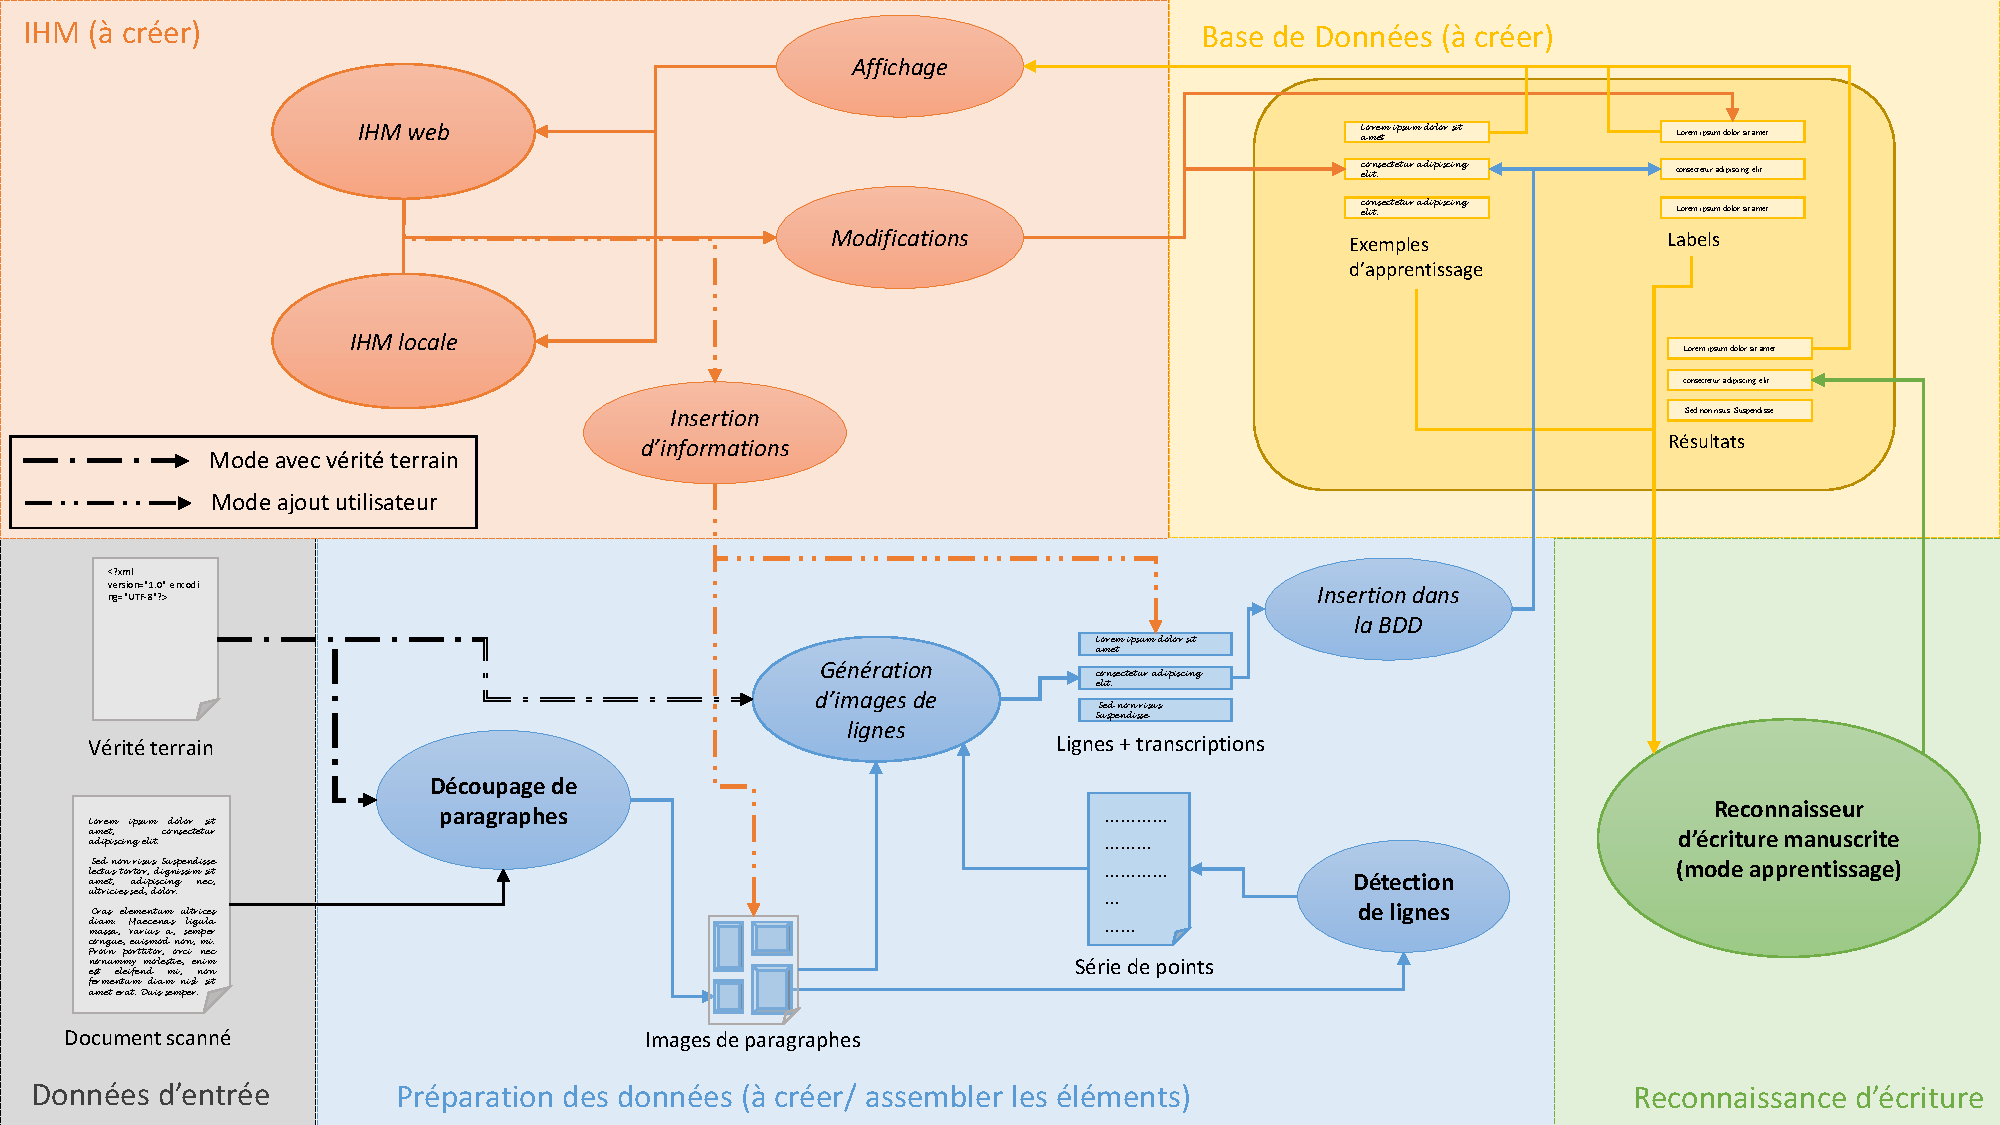
\includegraphics[width=\linewidth]{schema_mode1.1.pdf}
\end{center}
\end{mdframed}

\subsection{Traitement des documents en entrée}

Afin de générer des bases d’apprentissage, notre programme prendra en entrée des documents manuscrits
numérisés et leurs retranscriptions. On qualifie les retranscriptions de vérité terrain car elles
ont été réalisées par des humains et sont donc censées être justes. Le premier objectif est donc de
découper correctement les documents manuscrits sous la forme d’imagettes. Ces imagettes peuvent
correspondre à des lignes ou à des paragraphes des documents initiaux.

\paragraph{}
\begin{mdframed}[frametitle={Figure 3 : Exemple d'imagette}, innerbottommargin=10]
\begin{center}
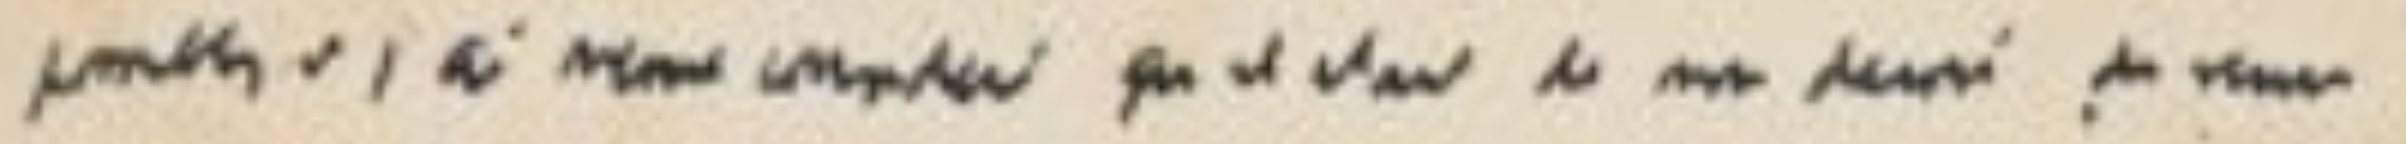
\includegraphics[width=\linewidth]{imagette.png}
\end{center}
\end{mdframed}

\paragraph{}
Le découpage en lignes se fait à l’aide de plusieurs outils : deux outils de détection de lignes qui nous sont fournis,
et un outil de découpage de paragraphes qui sera à développer au cours du projet. Cette partie correspond à la zone du
schéma sur fond bleu. Afin de générer les imagettes, nous avons deux possibilités :

\begin{itemize}
\item option détection sur le document (figure 4) : on détecte la position des lignes sur l’entièreté du document,
on découpe en paragraphes puis on relie les lignes détectées aux paragraphes;

\item option détection sur les paragraphes (figure 5) : on découpe d’abord les paragraphes, puis on détecte la position
des lignes dans chacun des paragraphes.
\end{itemize}

\paragraph{}
Ces deux possibilités ont des avantages et des inconvénients. La première possibilité a l’avantage d’être plus précise.
En effet, sur un document complet, on peut utiliser un meilleur outil de détection de lignes (à base de réseaux de
neurones à convolution) qui analyse la forme globale du document. L’inconvénient est qu’il faut relier les lignes
détectées à des paragraphes qui n’ont pas forcément une forme rectangulaire mais souvent plus complexe. Il faudra
donc utiliser des outils géométriques pour détecter l’appartenance d’un point à un polygone qui peut être concave.

\paragraph{}
La seconde possibilité est moins précise car l’outil de détection de lignes précédent ne peut pas s’appliquer
à un simple paragraphe. Nous devrons donc utiliser un autre outil (à base de floutage) qui peut traiter n’importe
quel format de document mais moins en détail. L’avantage de cette possibilité est que nous n’aurons pas à relier
les lignes aux paragraphes puisqu’elles y seront directement détectées. Nous avons cependant choisi d’implémenter
les deux possibilités pour rendre notre système compatible avec une plus grande variété de documents.

\paragraph{}
Le schéma représentant les objectifs du projet montre un mode de fonctionnement (partie en bleu) où
chaque imagette contient une seule ligne du document. Mais le projet doit contenir un second mode où
les imagettes représentent des paragraphes et où la partie détection de ligne est absente. Ce second
mode de fonctionnement permettra de générer des bases d’apprentissage pour des systèmes travaillant
sur des paragraphes entiers et non simplement sur des lignes. 

\paragraph{}
\begin{mdframed}[frametitle={Figure 4 : Partie traitement des données du projet (avec détection de lignes)}, innerbottommargin=10]
\begin{center}
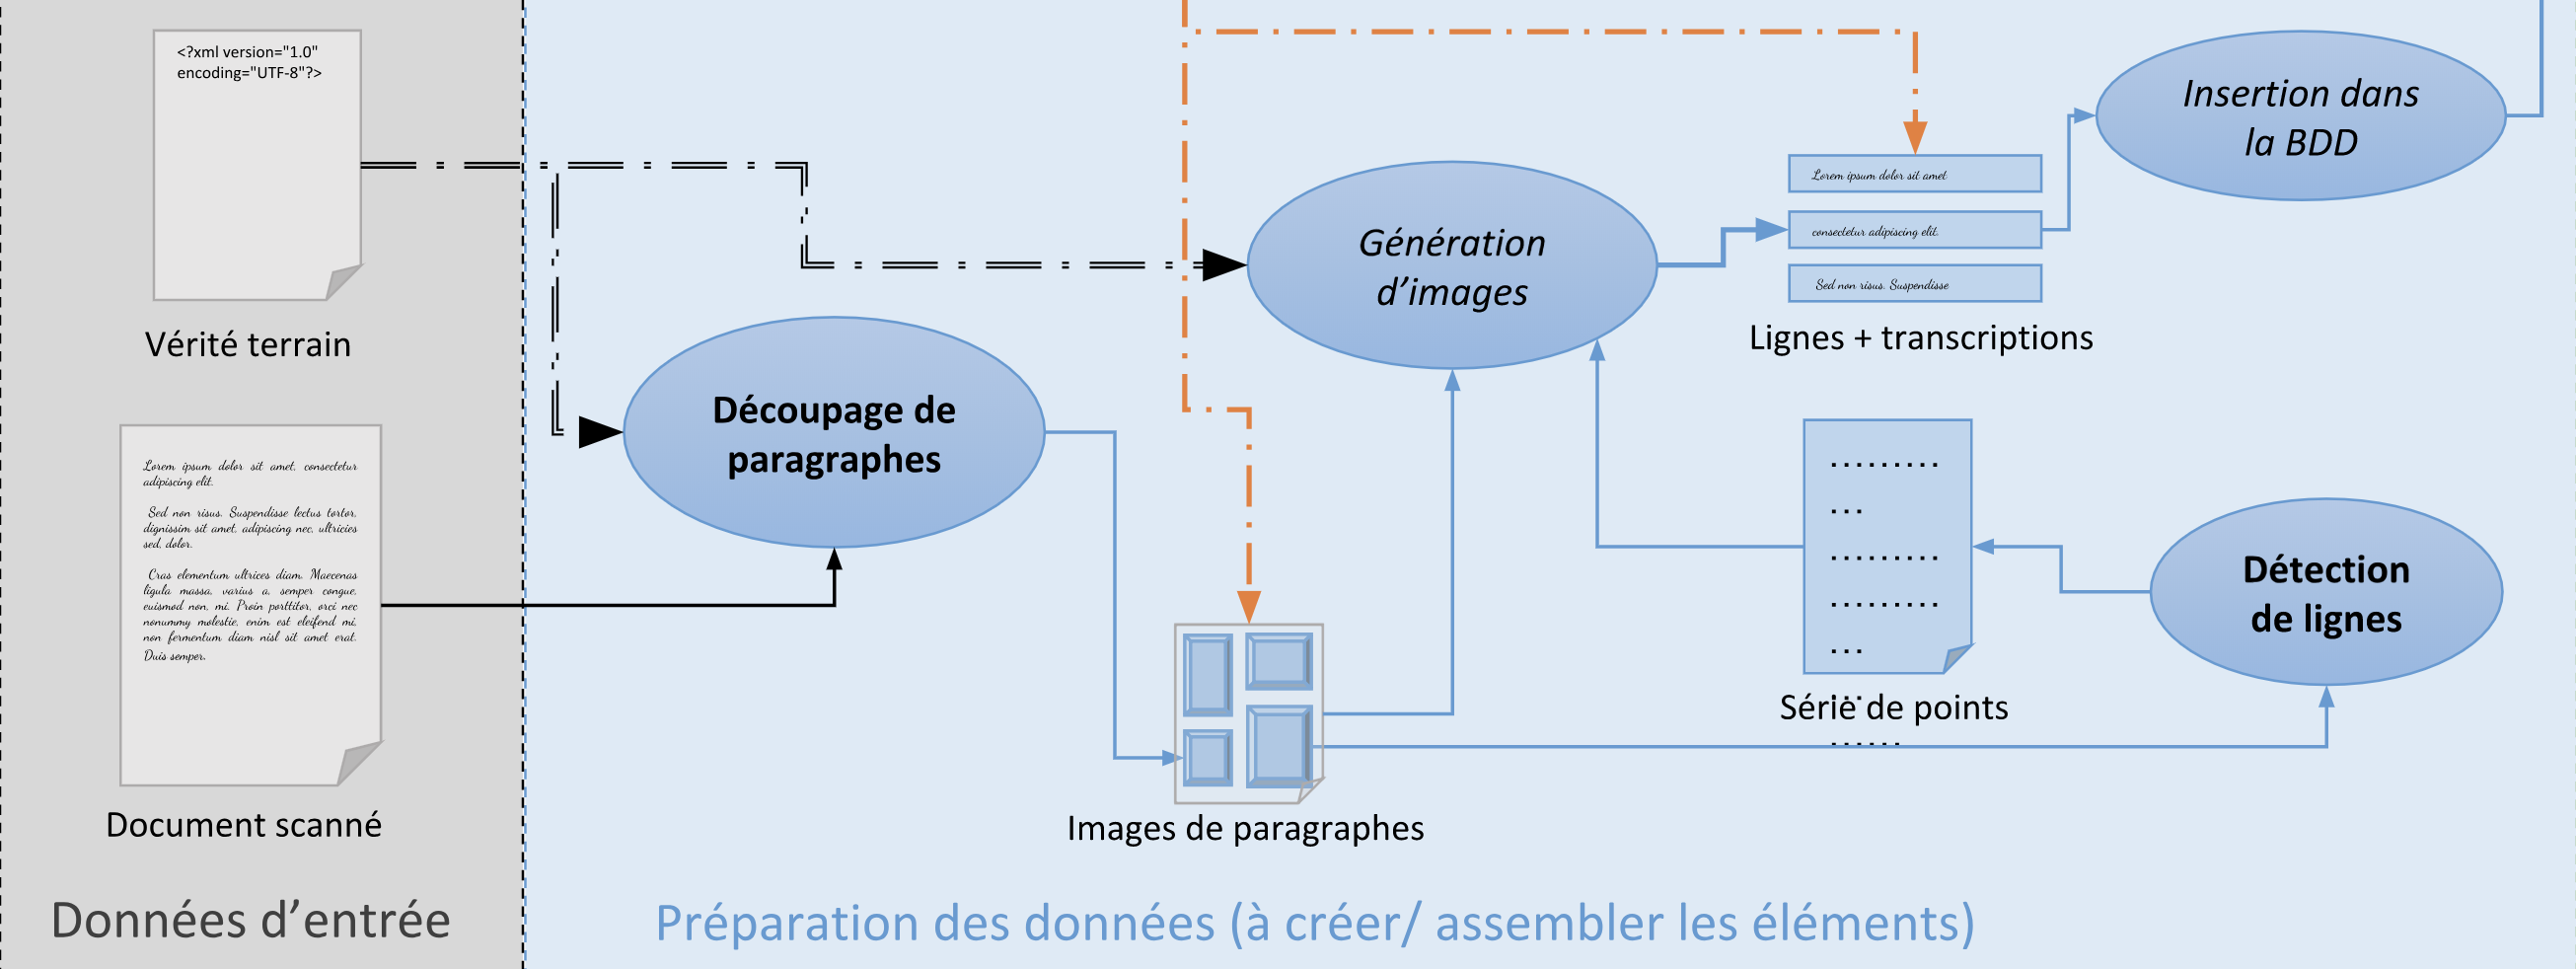
\includegraphics[width=\linewidth]{detection.png}
\end{center}
\end{mdframed}

\paragraph{}
\begin{mdframed}[frametitle={Figure 5 : Partie traitement des données du projet (sans détection de lignes)}, innerbottommargin=10]
\begin{center}
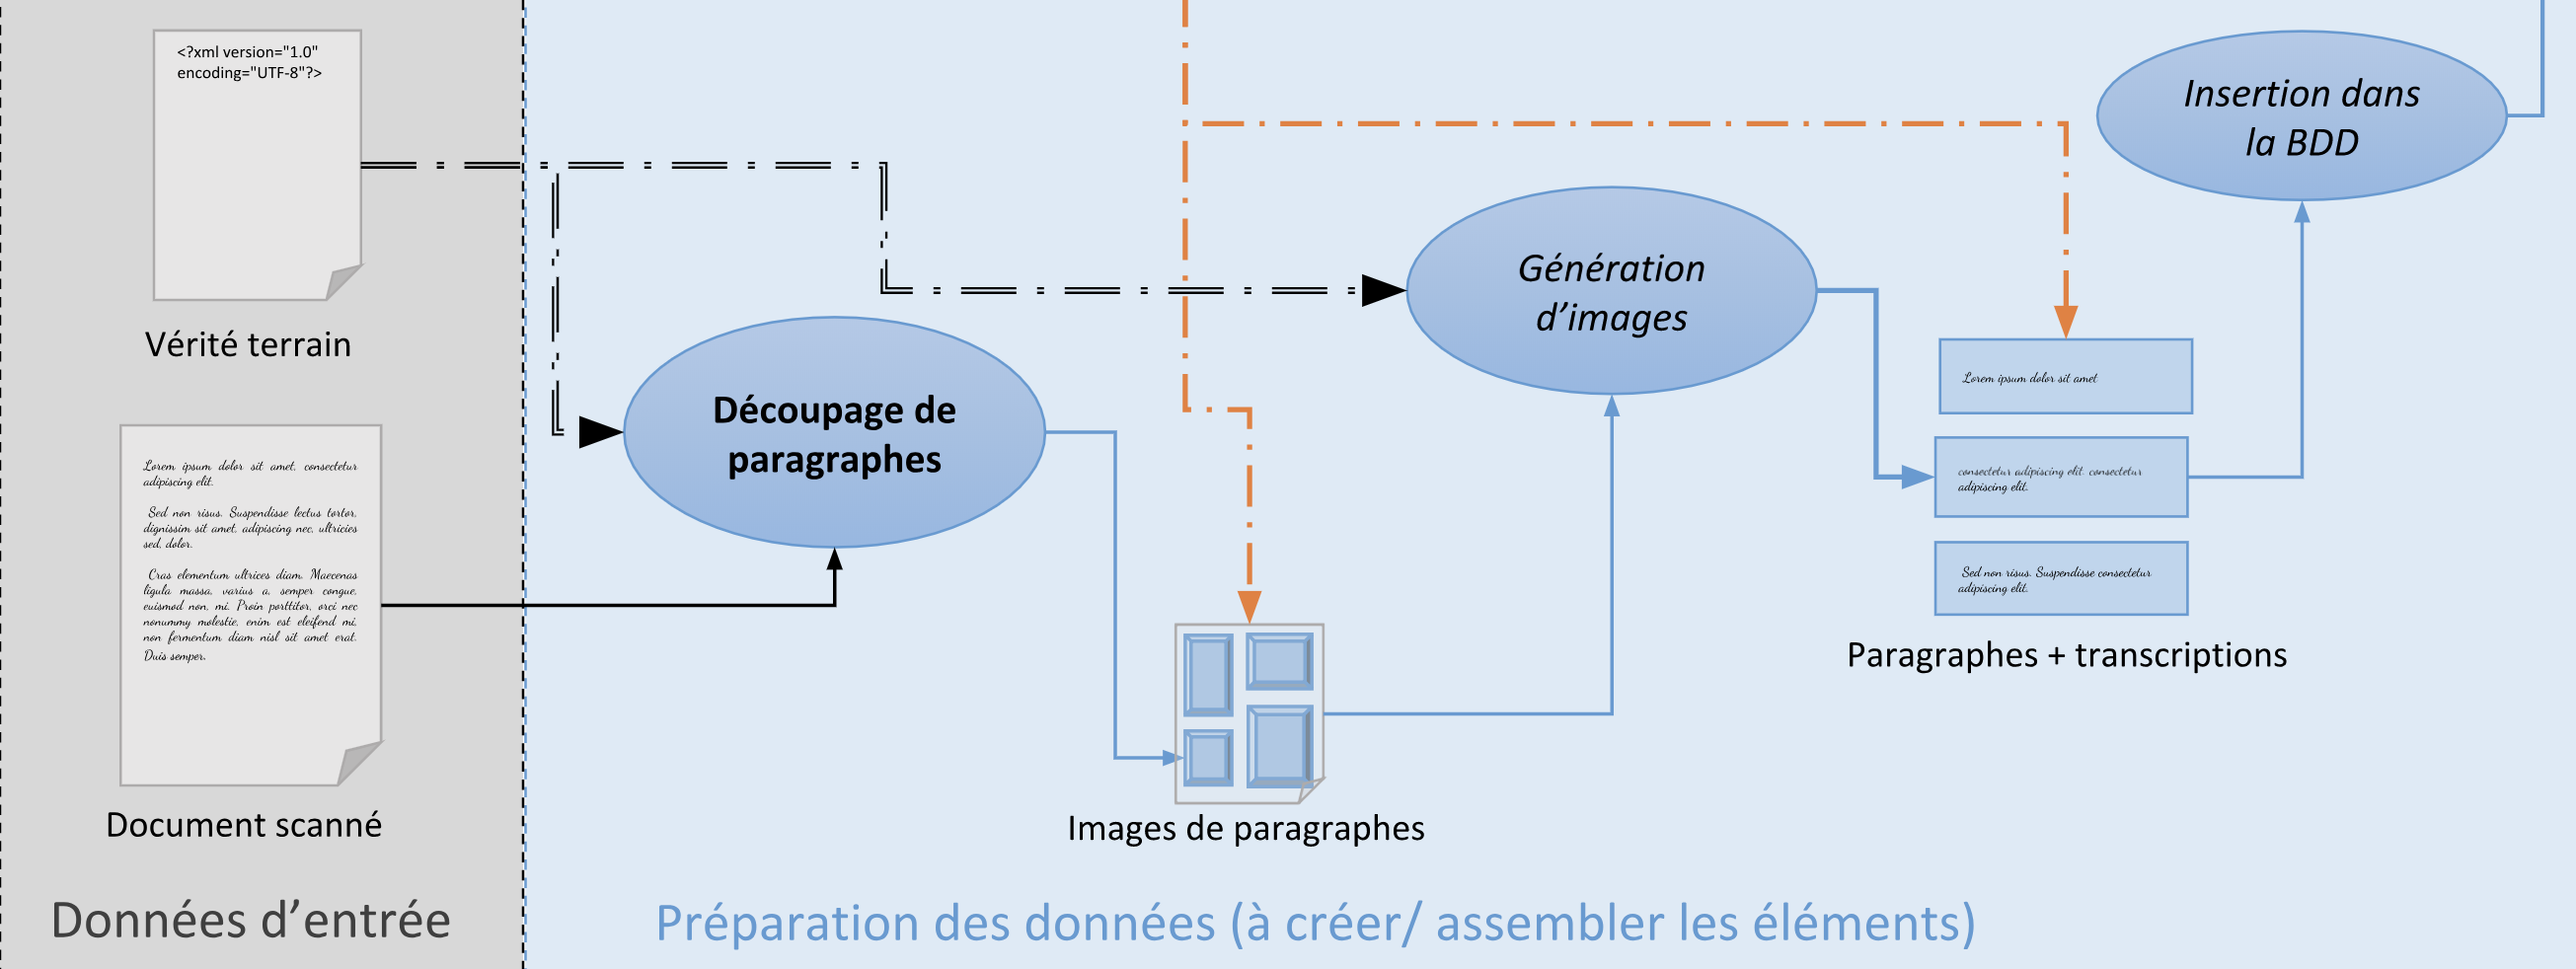
\includegraphics[width=\linewidth]{sans-detection.png}
\end{center}
\end{mdframed}

\paragraph{}
Dans un premier temps, nous travaillerons sur des documents provenant de la base
\href{http://www.maurdor-campaign.org/}{Maurdor}. Cette base, contenant des documents manuscrits numérisés
ainsi que leur retranscription, présente l’avantage d’avoir, en plus, les informations sur la position des
paragraphes et des retours à la ligne dans le document qui permettront de déduire la position des lignes
(tout cela dans un format spécifique dérivé du XML, le
\href{https://lampsrv02.umiacs.umd.edu/projdb/project.php?id=53}{format GEDI}). Nous utiliserons ces informations
pour découper les paragraphes. Par la suite, notre système devra être capable de prendre en entrée un autre
format de documents, le format PiFF\cite{piff:2017}, qui contient également les données de position des
paragraphes dans une image. Nous expliquerons pourquoi nous avons choisi ce format par la suite.

\subsection{Mise en relation des imagettes et de leur retranscription}

Afin que les imagettes puissent être exploitables, il faut les mettre en relation avec leur retranscription
numérique (contenue dans la vérité terrain). Cet objectif est réalisable grâces aux données de position qui accompagnent
les retranscriptions des fichiers d’entrée. Ces couples imagette-retranscription seront ensuite enregistrés
dans une base de données qui constituera la base d’apprentissage d’un système de reconnaissance d’écriture
manuscrite. Cette partie correspond également à la partie en bleu du schéma.

\subsection{Création d'une base de données}

La base de données contient donc les couples imagette-retranscription ainsi formés (partie jaune du schéma).
Il pourrait être intéressant de stocker, en plus, un texte généré par un reconnaisseur d’écriture pour
pouvoir tout conserver dans la même base.

\paragraph{}
La plupart des systèmes de \textit{deep learning} fonctionnent en trois modes : apprentissage, évaluation,
utilisation. Le système de reconnaissance d’écriture manuscrite est situé dans la partie verte du schéma.
La base de données que nous allons développer devra permettre de manipuler trois jeux de données différents : 

\begin{itemize}
\item tout d’abord, en mode d’apprentissage, notre logiciel extrait de la base les deux premiers jeux de données
(les imagettes et leurs retranscriptions associées) et les fournit au système de reconnaissance pour qu'il puisse s'entraîner;
\item ensuite, l'utilisateur doit pouvoir choisir un autre jeu de données pour évaluer son reconnaisseur; cela permet de vérifier
la qualité du reconnaisseur après un apprentissage; ainsi, si l'on utilise une seule base pour stocker les ensembles d’apprentissage
et d’évaluation, il pourrait être intéressant d’étiqueter les données pour indiquer dans quelle situation elles seront utilisées;
\item enfin, en mode de production, le reconnaisseur est supposé être bien entraîné; il n’a que les imagettes
en entrée et il fournit une retranscription numérique (un label) pour des documents sans vérité terrain;
il permet alors d’aider l’utilisateur à retranscrire numériquement un document manuscrit scanné; ce label généré pourrait donc
être intégré à la base de données commme nouvelle vérité terrain si l'utilisateur veut perfectionner son reconnaisseur.
\end{itemize}

\paragraph{}
Chaque mode de fonctionnement est illustré par un schéma en annexe A.

\subsection{Création d'une IHM permettant la modification de la base de données}

Il est possible que la vérité terrain ne soit pas toujours fournie en entrée ou qu’elle soit incorrecte.
Nous devons donc développer un logiciel permettant à l’utilisateur de rentrer lui-même une retranscription
numérique et de donner la position des paragraphes (mode ajout utilisateur sur le schéma). On doit également
pouvoir supprimer des couples imagette-retranscription de la base de données si jamais l’utilisateur considère
qu’elles n’apporteront rien de bénéfique à l’apprentissage du reconnaisseur. Les données qu’on pourrait vouloir
supprimer seraient des données trop bruitées, trop dégradées, mal coupées, etc. Il pourrait cependant être
intéressant de les conserver pour que le reconnaisseur apprenne à reconnaître des textes abîmés. Cet objectif
est représenté dans la partie rouge du schéma (IHM locale) qui doit pouvoir accéder à la base de données
et la modifier.

\subsection{Utiliser un format spécifique et convertible en sortie}

Notre logiciel générera des couples imagette-retranscription dans un format spécifique qui pourra ensuite être
facilement modifié, cela dans le but d’être compatible avec les formats d’entrée de plusieurs systèmes de
reconnaissance d’écriture manuscrite sans trop d’efforts. Plusieurs choix s’offrent à nous. Le format des données
en entrée de la base Maurdor est GEDI. Cependant, les formats d’autres bases sont différents. GEDI n’est donc pas
un format standard. Le format PiFF est un format de description d'images, mis en place par l'équipe IntuiDoc et par
d'autres laboratoires, qui se veut générique et facilement convertible dans d'autres formats. Il nous a donc paru
raisonnable de choisir d’utiliser ce format dans notre projet. Nous aurons donc un convertisseur du format d’entrée
GEDI en PiFF et un convertisseur de PiFF vers différents formats de librairies de \textit{deep learning}.

\subsection{Création d'une seconde IHM permettant d'observer les imagettes et les résultats d'un reconnaisseur}

Pour vérifier le bon fonctionnement de notre programme de génération de bases d’apprentissage, nous avons à notre
disposition un reconnaisseur d’écriture manuscrite nommé Laia\cite{laia:2016} dont nous parlerons plus tard.
Pour voir si notre système est efficace, il pourrait être intéressant de créer une seconde interface permettant
d’observer les imagettes et les résultats du reconnaisseur. Cet objectif est optionnel car il sort légèrement du
travail qui nous est demandé mais il sera utile pour faire une démonstration du reconnaisseur lors de la présentation
finale de notre projet. On pourra ainsi montrer ce que notre travail aura pu apporter à la reconnaissance d’écriture
manuscrite. Ce point ne sera probablement pas long à réaliser car il peut simplement consister en une amélioration
de l’IHM précédente. Pour rendre la démonstration plus ludique, on pourrait aussi créer une IHM sous forme de jeu
entre une personne et le reconnaisseur. Par exemple, la personne et le reconnaisseur pourraient avoir à retranscrire
un texte manuscrit le plus vite possible. Cet objectif est représenté dans la partie rouge du schéma (IHM web) qui
doit comme la première interface accéder à la base de données et la modifier.

\section{Description fonctionnelle des besoins}

\subsection{Diagramme bête à cornes}

Le diagramme de la figure 6 permet d’exprimer le besoin lié au projet. Ainsi, notre logiciel de
traitement de données manuscrites aura pour but principal de préparer et stocker des données
d’apprentissage pour des systèmes de reconnaissance d’écriture manuscrite.

\newpage

\paragraph{}
\begin{mdframed}[frametitle={Figure 6 : Diagramme bête à cornes}, innerbottommargin=10]
\begin{center}
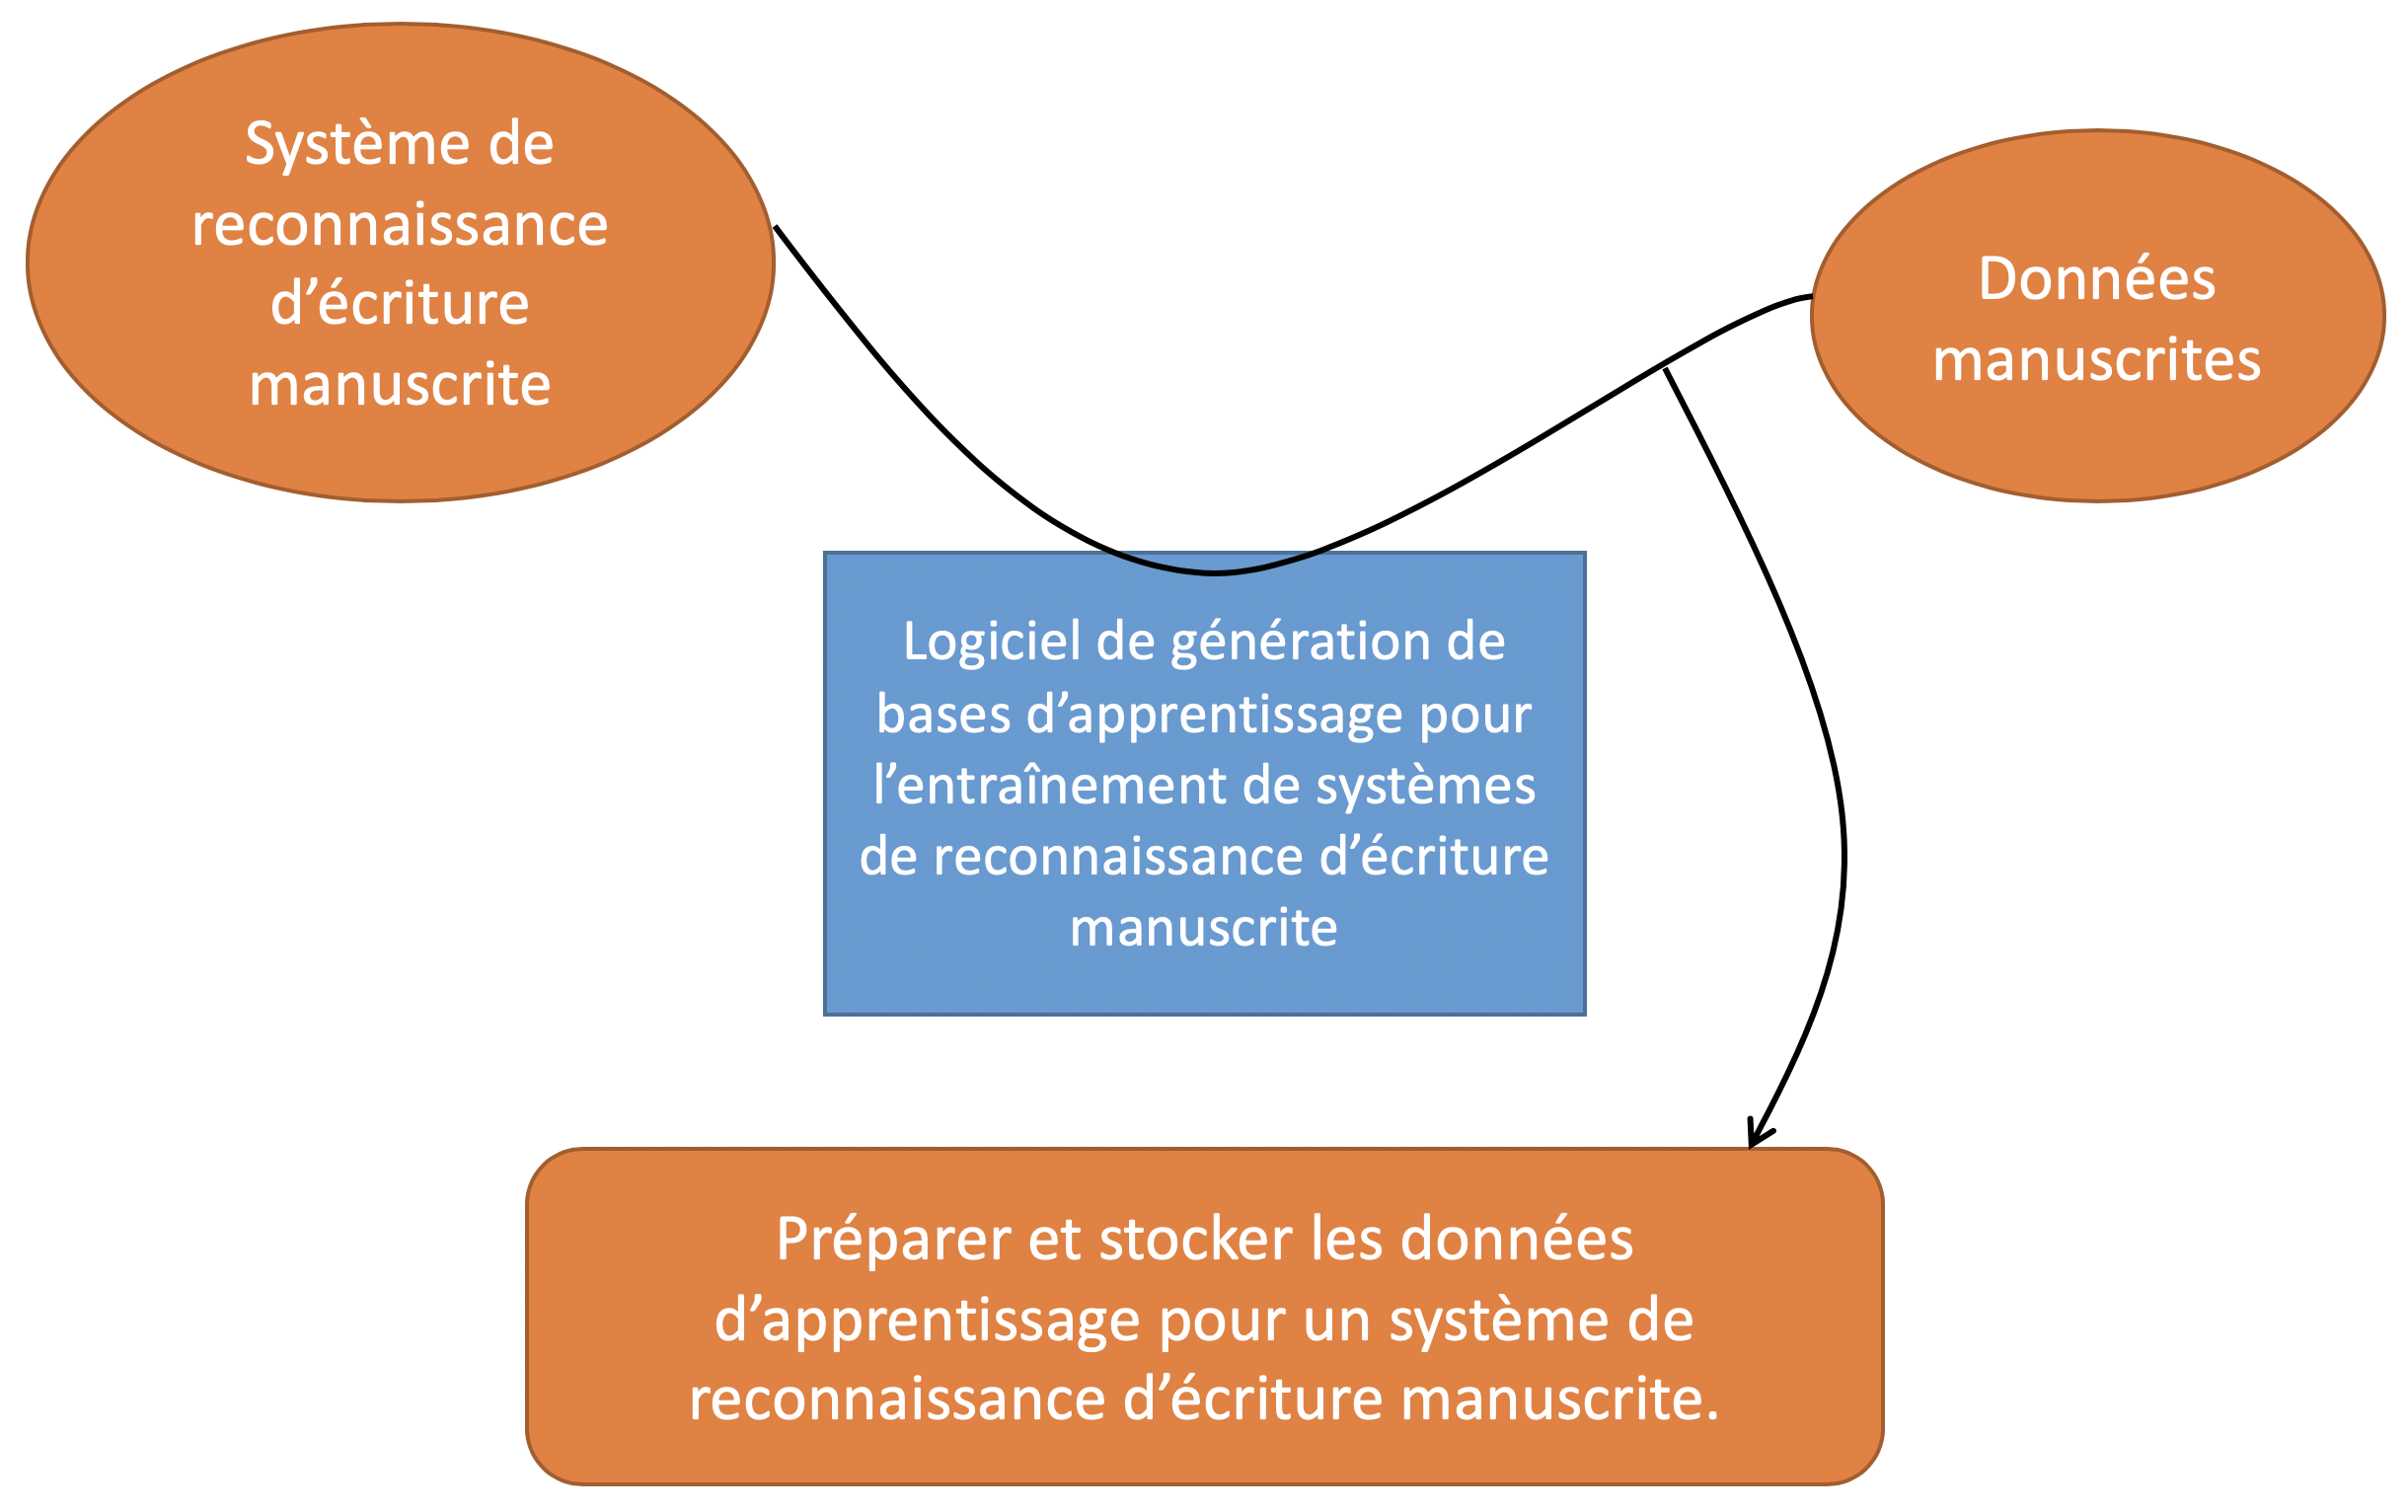
\includegraphics[width=0.6\linewidth]{bete-a-cornes.png}
\end{center}
\end{mdframed}

\subsection{Diagramme pieuvre}

Le diagramme pieuvre de la figure 7, quant à lui, permet d’exprimer les différentes fonctions contraintes
qui découlent de l’objectif principal du projet. De ce fait, notre logiciel devra interagir
avec différents acteurs afin de s’intégrer parfaitement dans l’optique du projet :

\begin{itemize}
\item \textbf{FP1} : tout d’abord, le premier objectif (et l’objectif principal du projet) est
de préparer et stocker les données d’apprentissage pour un système de reconnaissance d’écriture manuscrite;
\item \textbf{FC1} : ensuite, il devra utiliser le détecteur de lignes fourni afin de découper
les phrases des textes d’entrée en imagettes;
\item \textbf{FC2} : il devra également permettre à l’utilisateur d’interagir avec les données
traitées afin de les vérifier et/ou de les modifier si nécessaire, le tout par le biais d’une Interface Homme-Machine;
\item \textbf{FC3} : notre logiciel utilisera aussi la vérité terrain fournie afin d’associer
les imagettes découpées à la bonne transcription;
\item \textbf{FC4} : il faudra également que celui-ci soit compatible avec le format des données
qui lui seront fournies en entrée (format GEDI ou PiFF);
\item \textbf{FC5} : enfin, notre logiciel devra regrouper les données afin de les stocker dans une base de données.
\end{itemize}

\paragraph{}
\begin{mdframed}[frametitle={Figure 7 : Diagramme pieuvre}, innerbottommargin=10]
\begin{center}
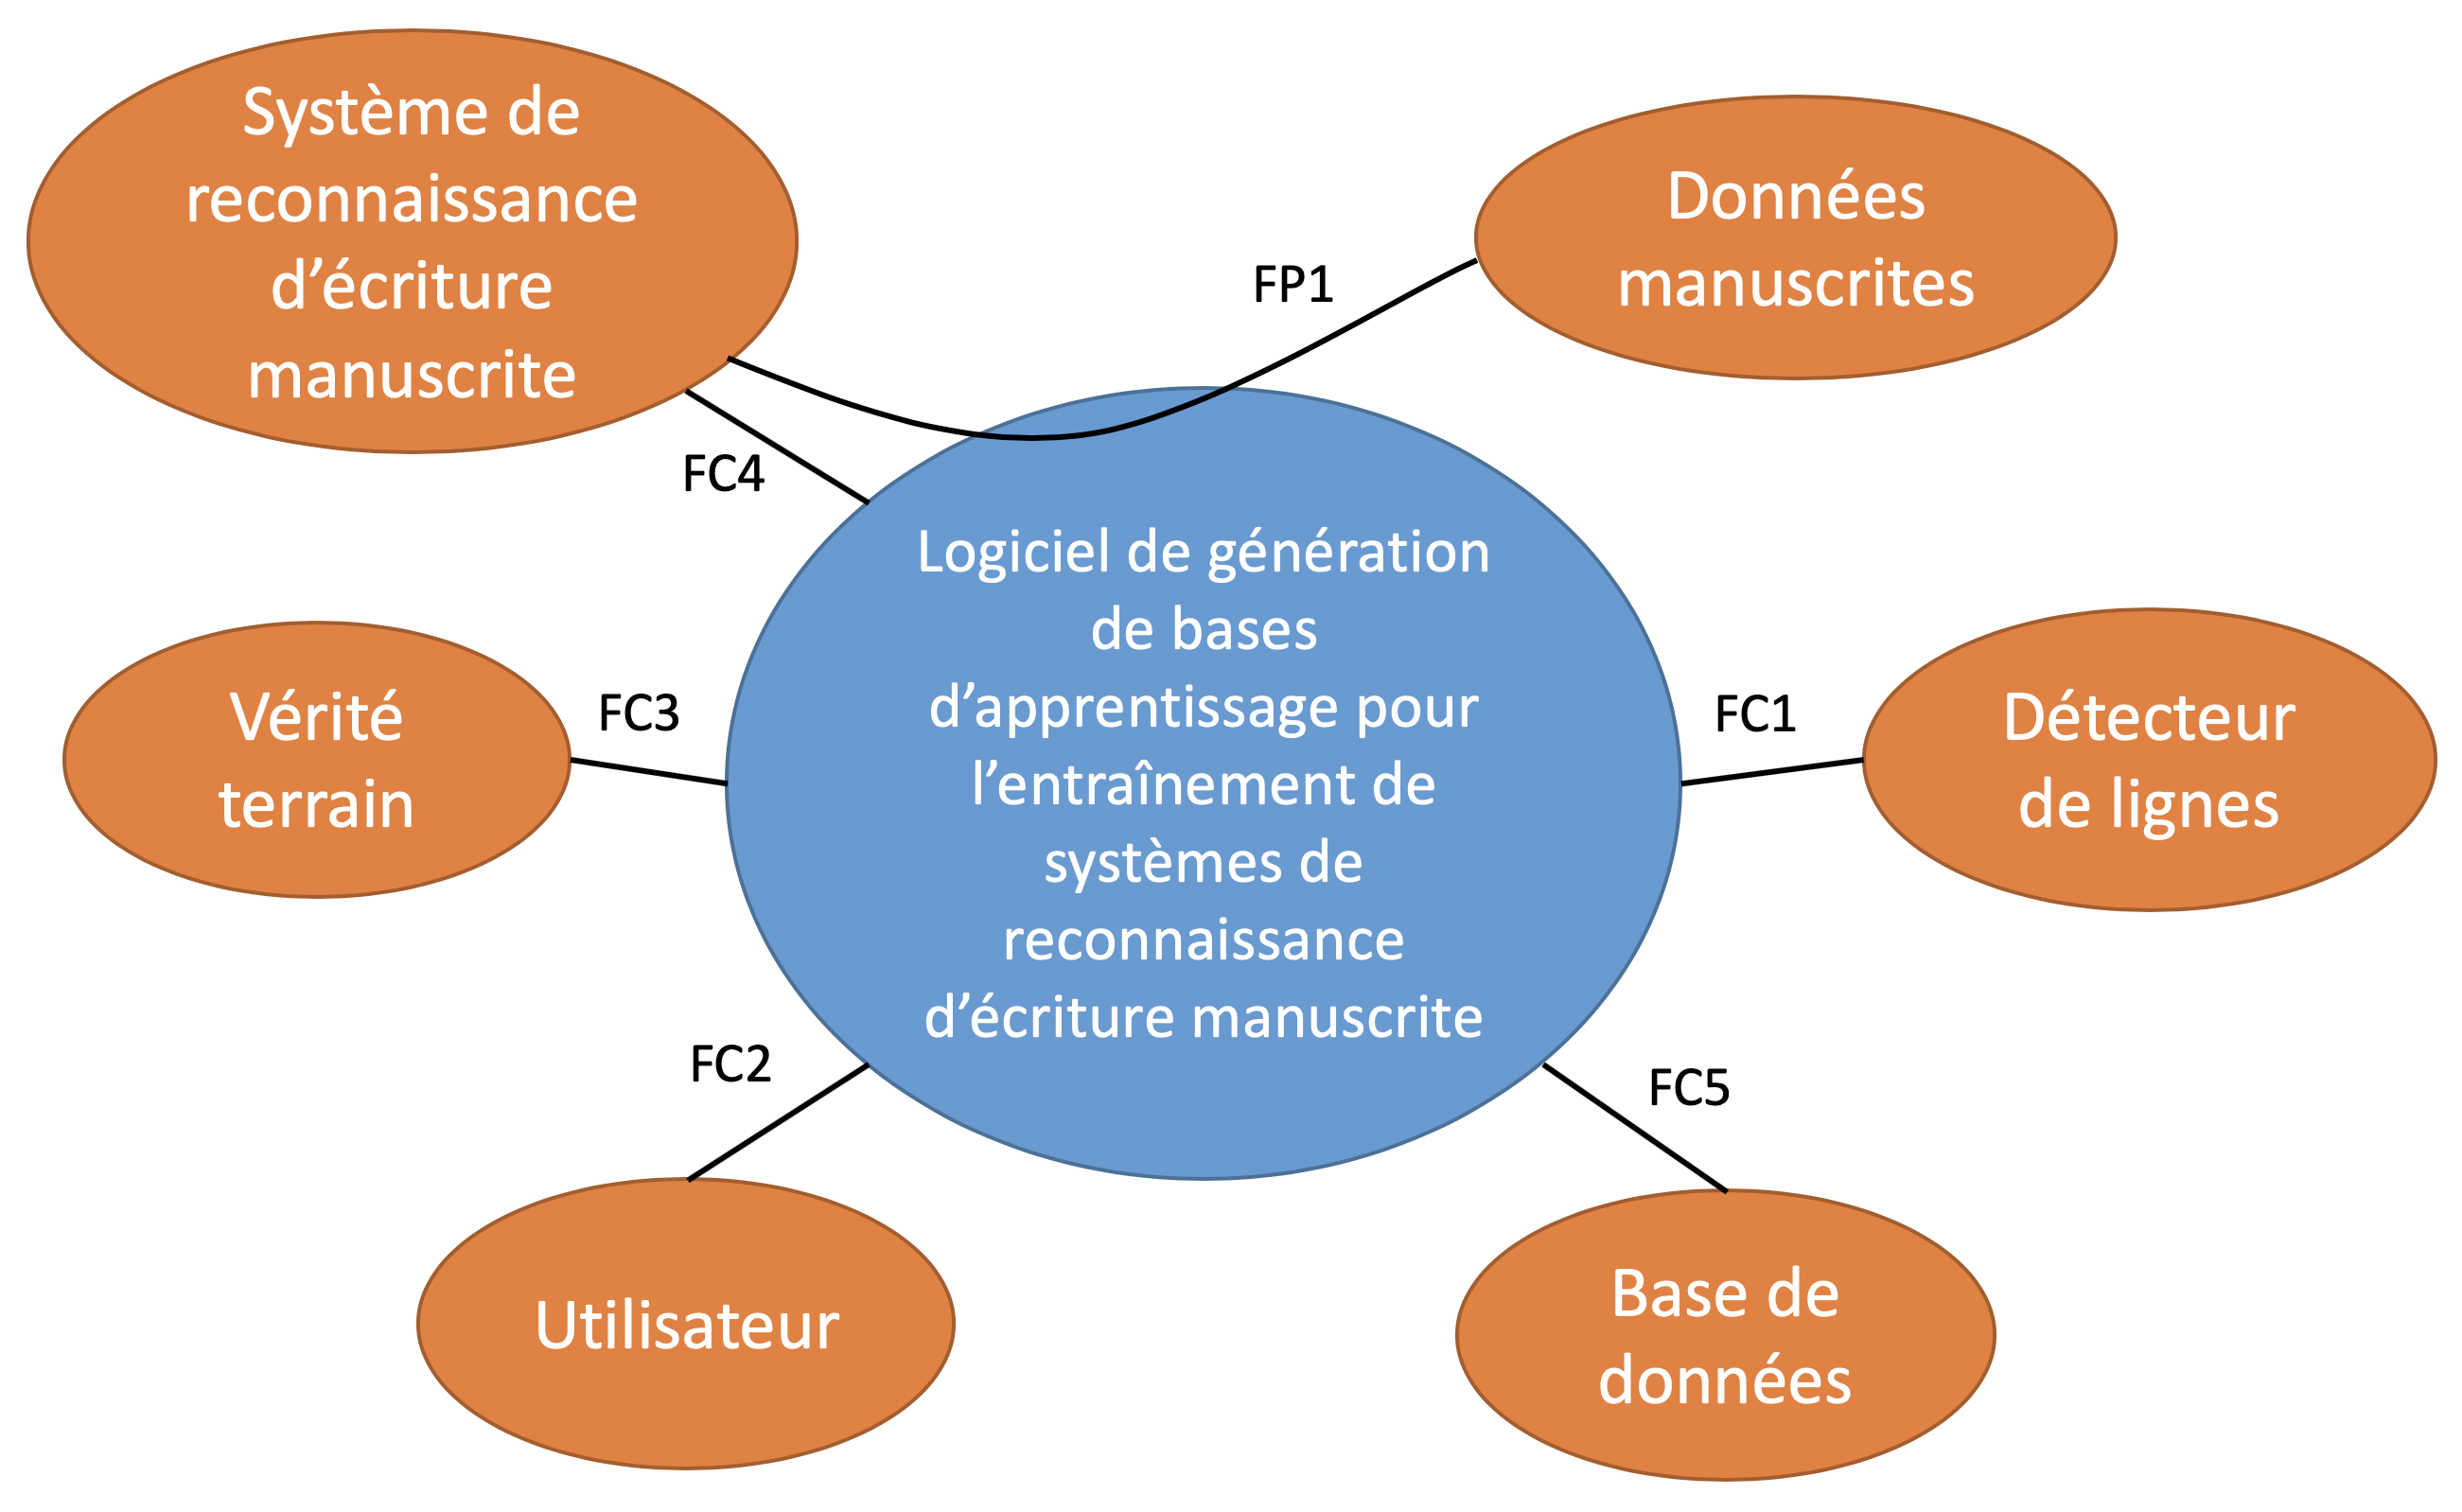
\includegraphics[width=0.6\linewidth]{pieuvre.png}
\end{center}
\end{mdframed}